% !TEX encoding = UTF-8 Unicode
\documentclass[a4paper,12pt]{article}
	
	% В этом документе преамбула
	
	%%% Работа с русским языком
	\usepackage{cmap}					% поиск в PDF
	\usepackage{mathtext} 				% русские буквы в формулах
	\usepackage[T2A]{fontenc}			% кодировка
	\usepackage[utf8]{inputenc}			% кодировка исходного текста
	\usepackage[english]{babel}	% локализация и переносы
	\usepackage{indentfirst}
	\frenchspacing
	
	\renewcommand{\epsilon}{\ensuremath{\varepsilon}}
	\renewcommand{\phi}{\ensuremath{\varphi}}
	\renewcommand{\kappa}{\ensuremath{\varkappa}}
	\renewcommand{\le}{\ensuremath{\leqslant}}
	\renewcommand{\leq}{\ensuremath{\leqslant}}
	\renewcommand{\ge}{\ensuremath{\geqslant}}
	\renewcommand{\geq}{\ensuremath{\geqslant}}
	\renewcommand{\emptyset}{\varnothing}
	
	%%% Дополнительная работа с математикой
	\usepackage{amsmath,amsfonts,amssymb,amsthm,mathtools} % AMS
	\usepackage{icomma} % "Умная" запятая: $0,2$ --- число, $0, 2$ --- перечисление
	
	%% Номера формул
	%\mathtoolsset{showonlyrefs=true} % Показывать номера только у тех формул, на которые есть \eqref{} в тексте.
	%\usepackage{leqno} % Нумереация формул слева
	
	%% Свои команды
	\DeclareMathOperator{\sgn}{\mathop{sgn}}
	
	%% Перенос знаков в формулах (по Львовскому)
	\newcommand*{\hm}[1]{#1\nobreak\discretionary{}
		{\hbox{$\mathsurround=0pt #1$}}{}}
	
	%%% Работа с картинками
	\usepackage{graphicx}  % Для вставки рисунков
	\setlength\fboxsep{3pt} % Отступ рамки \fbox{} от рисунка
	\setlength\fboxrule{1pt} % Толщина линий рамки \fbox{}
	\usepackage{wrapfig} % Обтекание рисунков текстом
	
	%%% Работа с таблицами
	\usepackage{array,tabularx,tabulary,booktabs} % Дополнительная работа с таблицами
	\usepackage{longtable}  % Длинные таблицы
	\usepackage{multirow} % Слияние строк в таблице
	
	%%% Теоремы
	\theoremstyle{plain} % Это стиль по умолчанию, его можно не переопределять.
	\newtheorem{theorem}{Theorem}
	\newenvironment{Proof} % имя окружения
	{\par\noindent{\bf Proof.}} % команды для \begin
	{\hfill$\scriptstyle\blacksquare$} % команды для \end
	
	\newtheorem{proposition}[theorem]{Утверждение}
	
	\theoremstyle{definition} % "Определение"
	\newtheorem{corollary}{Следствие}[theorem]
	\newtheorem{problem}{Задача}[section]
	
	\theoremstyle{remark} % "Примечание"
	\newtheorem*{nonum}{Решение}
	
	%%% Программирование
	\usepackage{etoolbox} % логические операторы
	
	%%% Страница
	\usepackage{extsizes} % Возможность сделать 14-й шрифт
	\usepackage{geometry} % Простой способ задавать поля
	\geometry{top=25mm}
	\geometry{bottom=35mm}
	\geometry{left=35mm}
	\geometry{right=20mm}
	%
	%\usepackage{fancyhdr} % Колонтитулы
	% 	\pagestyle{fancy}
	%\renewcommand{\headrulewidth}{0pt}  % Толщина линейки, отчеркивающей верхний колонтитул
	% 	\lfoot{Нижний левый}
	% 	\rfoot{Нижний правый}
	% 	\rhead{Верхний правый}
	% 	\chead{Верхний в центре}
	% 	\lhead{Верхний левый}
	%	\cfoot{Нижний в центре} % По умолчанию здесь номер страницы
	
	\usepackage{setspace} % �?нтерлиньяж
	%\onehalfspacing % �?нтерлиньяж 1.5
	%\doublespacing % �?нтерлиньяж 2
	%\singlespacing % �?нтерлиньяж 1
	
	\usepackage{lastpage} % Узнать, сколько всего страниц в документе.
	
	\usepackage{soul} % Модификаторы начертания
	
	\usepackage{hyperref}
	\usepackage[usenames,dvipsnames,svgnames,table,rgb]{xcolor}
	\hypersetup{				% Гиперссылки
		unicode=true,           % русские буквы в раздела PDF
		pdftitle={Заголовок},   % Заголовок
		pdfauthor={Автор},      % Автор
		pdfsubject={Тема},      % Тема
		pdfcreator={Создатель}, % Создатель
		pdfproducer={Производитель}, % Производитель
		pdfkeywords={keyword1} {key2} {key3}, % Ключевые слова
		colorlinks=true,       	% false: ссылки в рамках; true: цветные ссылки
		linkcolor=red,          % внутренние ссылки
		citecolor=black,        % на библиографию
		filecolor=magenta,      % на файлы
		urlcolor=blue           % на URL
	}
	
	\usepackage{csquotes} % Еще инструменты для ссылок
	
	%\usepackage[style=authoryear,maxcitenames=2,backend=biber,sorting=nty]{biblatex}
	
	\usepackage{multicol} % Несколько колонок
	
	\usepackage{tikz} % Работа с графикой
	\usepackage{pgfplots}
	\usepackage{pgfplotstable}
	
	\usepackage{algorithm}
	\usepackage[noend]{algcompatible}
	
	\newcommand{\ba}{\mathbf{a}}
	\newcommand{\bb}{\mathbf{b}}
	\newcommand{\bw}{\mathbf{w}}
	\newcommand{\by}{\mathbf{y}}
	\newcommand{\bx}{\mathbf{x}}
	\newcommand{\bz}{\mathbf{z}}
	\newcommand{\cA}{\mathcal{A}}
	\newcommand{\bJ}{\mathbf{J}}
	\newcommand{\bQ}{\mathbf{Q}}
	\newcommand{\bbR}{\mathbb{R}}
	\newcommand{\bW}{\mathbf{W}}
	\newcommand{\bY}{\mathbf{Y}}
	\newcommand{\bX}{\mathbf{X}}
	
	\newcommand{\T}{{\text{\tiny\sffamily\upshape\mdseries T}}}
	\newcommand{\argmin}{\mathop{\arg \min}\limits}
	\newcommand{\argmax}{\mathop{\arg \max}\limits}
	
	\usepackage{tikz-cd}
	
	\begin{document}
		
	\section*{Problem Statement}

	We consider the regression problem of predicting an target variable $y \in \bbR$ given an object $\bx \bbR^{n}$. 
	The goal is to build a model $f(\bx | \bw), \bw \in \mathbb{R}^p$ which outcomes a prediction for each input object.
	Let assume that we are given the design matrix~$\bX = [\bx_1, \dots, \bx_m]^{\T} \in \bbR^{m \times n}$ and the target vector~$\by = [y_1, \dots, y_m]^{\T} \in \bbR^{m}$. 
	Each $i$-th matrix~$\bX$ row represents an object which is associated with the $i$-th vector~$\by$ element.
	The goal is to find the optimal weight vector $\bw^*$.
	
	The weights~$\bw$ are fitted by the minimization of an error function:
	\begin{equation}
	\bw^* = \argmin_{\bw \in \bbR^r} S(\bw | \bX, \by, f).
	\label{eq:error_function}
	\end{equation}
	The most common choice for the error function~$S(\bw | \bX, \by, f)$ in the regression task is the squared error between real target values and predicted ones
	\[
		S(\bw | \bX, \by, f) =  \| \by - \mathbf{f}(\bX | \bw)\|_2^2 = \sum_{i=1}^m (y_i - f(\bx_i | \bw))^2.
	\]

	The problem~\ref{eq:error_function} could be solved by any neural network optimization method~[].
	
	The number of model weights~$p$ could be extremely huge. 
	In this case the solution of the problem~\ref{eq:error_function} leads to overfitting. 
	To eliminate this problem we propose to select the subset~$\cA \subseteq \{1, \dots, p\}$ of the active weights. 
	The weights which are not active are supposed to be zero.
	To choose the subset~$\cA$ from all possible $2^p$ combinations let introduce a quality criteria~$Q(\cA | \bX, \by, f)$. 
	This function evaluates the quality of a particular active set $\cA$. 
	We desire to find the optimal subset $\cA^*$ which minimizes the quality criteria
	\begin{equation}
		\cA^* = \argmin_{\cA \subseteq \{1, \dots, p\}} Q(\cA | \bX, \by, f).
		\label{eq:quality_criteria}
	\end{equation}
	
	If the solution $\cA^*$ of the~\ref{eq:quality_criteria} is given the next step is to determine the optimal model weights	$\bw^*$ by solving a problem
	
	\begin{equation}
		\bw^* = \argmin_{\bw \in \bbR^p} S(\bw | \bX, \by, f), \quad \text{subject to } w_j = 0 \text{ for } j \notin \cA^*.
		\label{eq:reduced_error_function}
	\end{equation}
	
	\section*{QPFS}
	
	To find the optimal subset $\cA^*$ we suggest to use QPFS algorithm.
	The original algorithm selects features for the linear regression task, where the model $f(\bx | \bw) = \bx^{\T} \bw$ and the problem~\ref{eq:error_function}
	\[
		S(\bw | \bX, \by, f) =  \| \by - \bX \bw\|_2^2 \rightarrow\min_{\bw \in \bbR^{n}}.
	\]
	The goal of the QPFS is to select not correlated features which are relevant to target vector.
	To formalise this approach let introduce two functions: Sim and Rel. 
	The former measures the redundancy between features, the latter contains relevances between each feature and target vector. 
	We want to minimize the Sim function and maximize the Rel simultaneously.
	
	The QPFS method offers the explicit way to construct the functions Sim and Rel. 
	The method minimizes the following functional
	\begin{equation}
		\underbrace{\bz^{\T} \bQ \bz}_{\text{Sim}} - \alpha \cdot \underbrace{\vphantom{()} \mathbf{b}^{\T} \bz}_{\text{Rel}} \rightarrow \min_{\bz \in [0, 1]^n}.
		\label{eq:quadratic_problem}
	\end{equation}
	This functional is an analogue of the described quality criteria~\ref{eq:quality_criteria}.
  	The first term is associated with the Sim function and the second with the Rel. 
  	The matrix $\bQ \in \bbR^{n \times n}$ entries measure the pairwise similarities between features. 
  	The vector $\mathbf{b} \in \bbR^n$ expresses the similarities between each feature and the target vector~$\by$.
  	The normalized vector~$\bz$ shows the importance of each feature. 
  	This functional penalizes the dependent features by the function Sim and encourages features relevant to the target by the function Rel. 
  	The parameter $\alpha$ allows to control the trade-off between the Sim and the Rel terms.
  	To find the optimal feature subset the thresholding for $\bz$ is applied:
  	\[
  		j \in \mathcal{A} \Leftrightarrow z_j > \tau.
  	\]
  	
  	To measure similarity it was proposed to use the absolute value of sample Pearson correlation coefficient or sample mutual information between pairs of features for the Sim function and between features and target vector for the Rel function.
  	The problem~\ref{eq:quadratic_problem} is convex if the matrix~$\bQ$ is positive semidefinite. In general it is not always true. 
  	To satisfy this condition we shift the matrix $\bQ$ spectrum and replace the matrix~$\bQ$ by $\bQ - \lambda_{\text{min}} \mathbf{I}$, where $\lambda_{\text{min}} $ is a $\bQ$ minimal eigenvalue.
  	
  	\section*{Model linearization}
  	Let assume that we have the model $f(\bx | \bw)$ and the weight vector $\bw$ and we want to find the new weights by adding the updates $\Delta \bw$ to the existing weights $\bw$. 
  	Similar to the Levenberg-Marquardt algorithm, we use the linear approximation of the model
  	\[
	  	\mathbf{f}(\bX | \bw + \Delta \bw) \approx \mathbf{f}(\bX | \bw) + \bJ \cdot \Delta  \bw,
	\]
	
	where $\mathbf{J} \in \bbR^{m \times p}$ is a Jacobian matrix
	\begin{equation}
		\bJ = 
		\begin{pmatrix}
		\frac{\partial f(\bx_1 | \bw)}{\partial w_1} & \dots & 
		\frac{\partial f(\bx_1 | \bw)}{\partial w_p} \\
		\dots & \dots & \dots \\
		\frac{\partial f(\bx_m | \bw)}{\partial w_1} & \dots & 
		\frac{\partial f(\bx_m | \bw)}{\partial w_p}
		\end{pmatrix}.
	\end{equation}
	In this case the problem~\ref{eq:error_function} is a linear regression problem with the target vector $\by - \mathbf{f}(\bX | \bw)$, matrix $\bJ$ and weights $\Delta \bw$
	\begin{equation}
		S(\bw + \Delta \bw | \bX, \by, f) =  \| \by - \mathbf{f}(\bX | \bw + \Delta \bw)\|_2^2 \approx  \| (\by - \mathbf{f}(\bX | \bw)) - \bJ \cdot \Delta  \bw\|_2^2.
	\label{eq:qpfs_nn}
	\end{equation}
  	To find the most significant set of weights for the current point $\bw$ we can apply QPFS algorithm. 
  	Significance means the relevance of the weight update to the residual vector and pairwise weights updates independence through training data.
  	
  	We use backpropagation procedure to update the network weights. 
  	The most of the neural network optimization methods use the gradient of the model to update network weights. 
  	It allows to get the Jacobian matrix $\bJ$ for free from optimization process. 
  	
  	We want to investigate the dependence of the QPFS solution for the problem~\ref{eq:qpfs_nn}. 
  	Let assume that we have some weight vector~$\bw^0$ which lies near the optimal weight vector~$\bw^*$. 
  	We consider the line segment
  	\[
  		\bw_{\beta} = \beta \bw^* + (1 - \beta) \bw^0; \, \beta \in [0, 1] .
  	\]
  	
  	\subsection*{Linear model}
  	In the case of linear model $f(\bx | \bw) = \bx^{\T} \bw$, the Jacobian matrix~$\bJ$ equals the design matrix~$\bX$. 
  	The problem~\ref{eq:qpfs_nn} has the form
  	\[
  		 \| (\by - \mathbf{f}(\bX | \bw)) - \bJ \cdot \Delta  \bw\|_2^2 = \| (\by - \bX \bw) - \bX \cdot \Delta  \bw\|_2^2.
  	\]
  	
  	The matrix $\bQ$ entries are the similarities between features, the vector $\bb$ entries are the feature relevances to the residual vector $\by - \bX \bw$. 
  	Therefore, the $\bQ$ matrix is constant with respect to the model weights $\bw$. 
  	The vector $\bb$ entries decreases as the $\beta$ coefficient is getting smaller. The residual vector $\by - \bX \bw^*$ is orthogonal to the matrix $\bX$ columns for the optimal weights $\bw^*$, since the correlation and the mutual information coefficients equals zero for the orthogonal vectors.
  	
  	\subsection*{Two layer neural network}
  	We consider the feed-forward two layer neural network as the nonlinear model. In this case the model~$f(\bx | \bw)$ is given by
  	\[
  		f(\bx | \bw) = \sigma(\bx^{\T} \bW_1) \bW_2.
  	\]
  	Here~$\bW_1 \in \bbR^{n \times h}$ the weight matrix which connects the input features with $h$ hidden units, $\sigma(\cdot)$ is a nonlinearity function which applied element-wise, and $\bW_2 \in \bbR^{h \times 1}$ the weight matrix which connects the hidden units with output. 
  	The model weight vector~$\bw$ is a concatenation of vectorized matrices~$\bW_1$, $\bW_2$.
  	
  	The first order optimization condition tells that in the optimal point the first derivatives of the error function are equal to
  	\[
  		\left.\frac{\partial S(\bw | \bX, \by, f)}{\partial \bw} \right|_{\bw = \bw^*}=  (\by - \mathbf{f}(\bX | \bw))^{\T} \mathbf{J}\Bigr|_{\bw=\bw^*} = 0.
  	\]
  	This implies the orthogonality between residual vector $\by - \mathbf{f}(\bX | \bw)$ and the columns of the Jacobian matrix $\bJ$. It means that in the optimum point $\bw^*$ the linear term $\bb$ will be around zero. 
  	
  	\section*{Experiment}
  	In the experiment we used the Boston House Pricing dataset (objects: 506, features: 13). 
  	
  	First of all we investigate the influence of $\alpha$ coefficient to the QPFS function~\ref{eq:quadratic_problem}. Figure~\ref{fig:qpfs_corr_vs_info_wrt_alpha} shows the features scores $\bz \in \bbR^{13}$ for correlation and mutual information coefficients with respect to different $\alpha$. If $\alpha$ is large enough the Rel term is prevailed. All features is active in this case. The algorithm does not penalize features and selects features relevant to the target. As $\alpha$ goes down the Sim term starts to penalize feature interactions and the active set of features shrinks. It worth to note that correlations mutual information works in different ways.
  	
  	\begin{figure}[h]
  		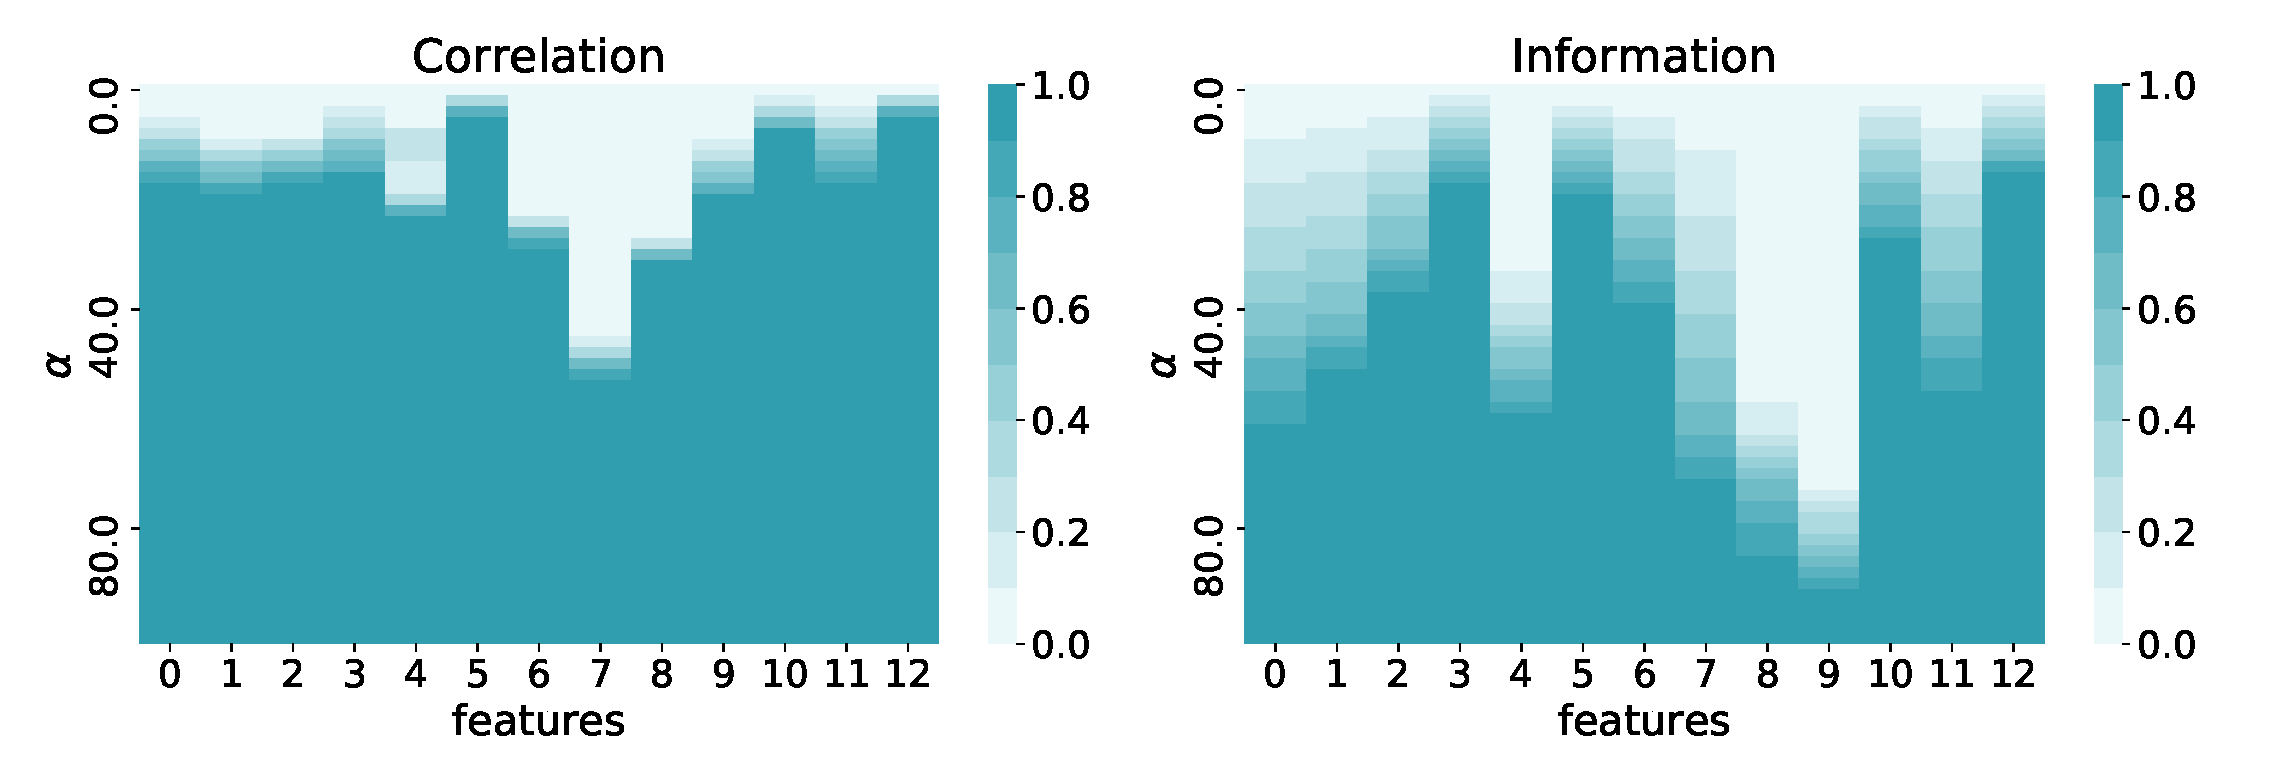
\includegraphics[width=\linewidth]{figs/qpfs_corr_vs_info_wrt_alpha.eps}
  		\caption{QPFS scores with respect to $\alpha$ coefficient}
  		\label{fig:qpfs_corr_vs_info_wrt_alpha}
  	\end{figure}
  
  The authors of the original QPFS paper suggested the way to select $\alpha$ and make Sim and Rel terms impact are equal
  \[
  	\alpha = \frac{\overline{\bQ}}{\overline{\bQ} + \overline{\bb}},
  \] 
  where $\overline{\bQ}$, $\overline{\bb}$ are the mean values of $\bQ$ and $\bb$ correspondingly.
  
  We fitted the linear model for this data.
  The error landscape is shown in the figure~\ref{fig:linear_error} for two randomly selected weights. 
  We add the random noise to the optimum weights $\bw^*$ to get the point $\bw^0$. The behaviour of the Rel term vector $\bb$ on the line segment between $\bw^0$ and $\bw^*$ is illustrated in the figure~\ref{fig:linear_b_wrt_beta}.

	\begin{figure}[!h]	
		\centering
		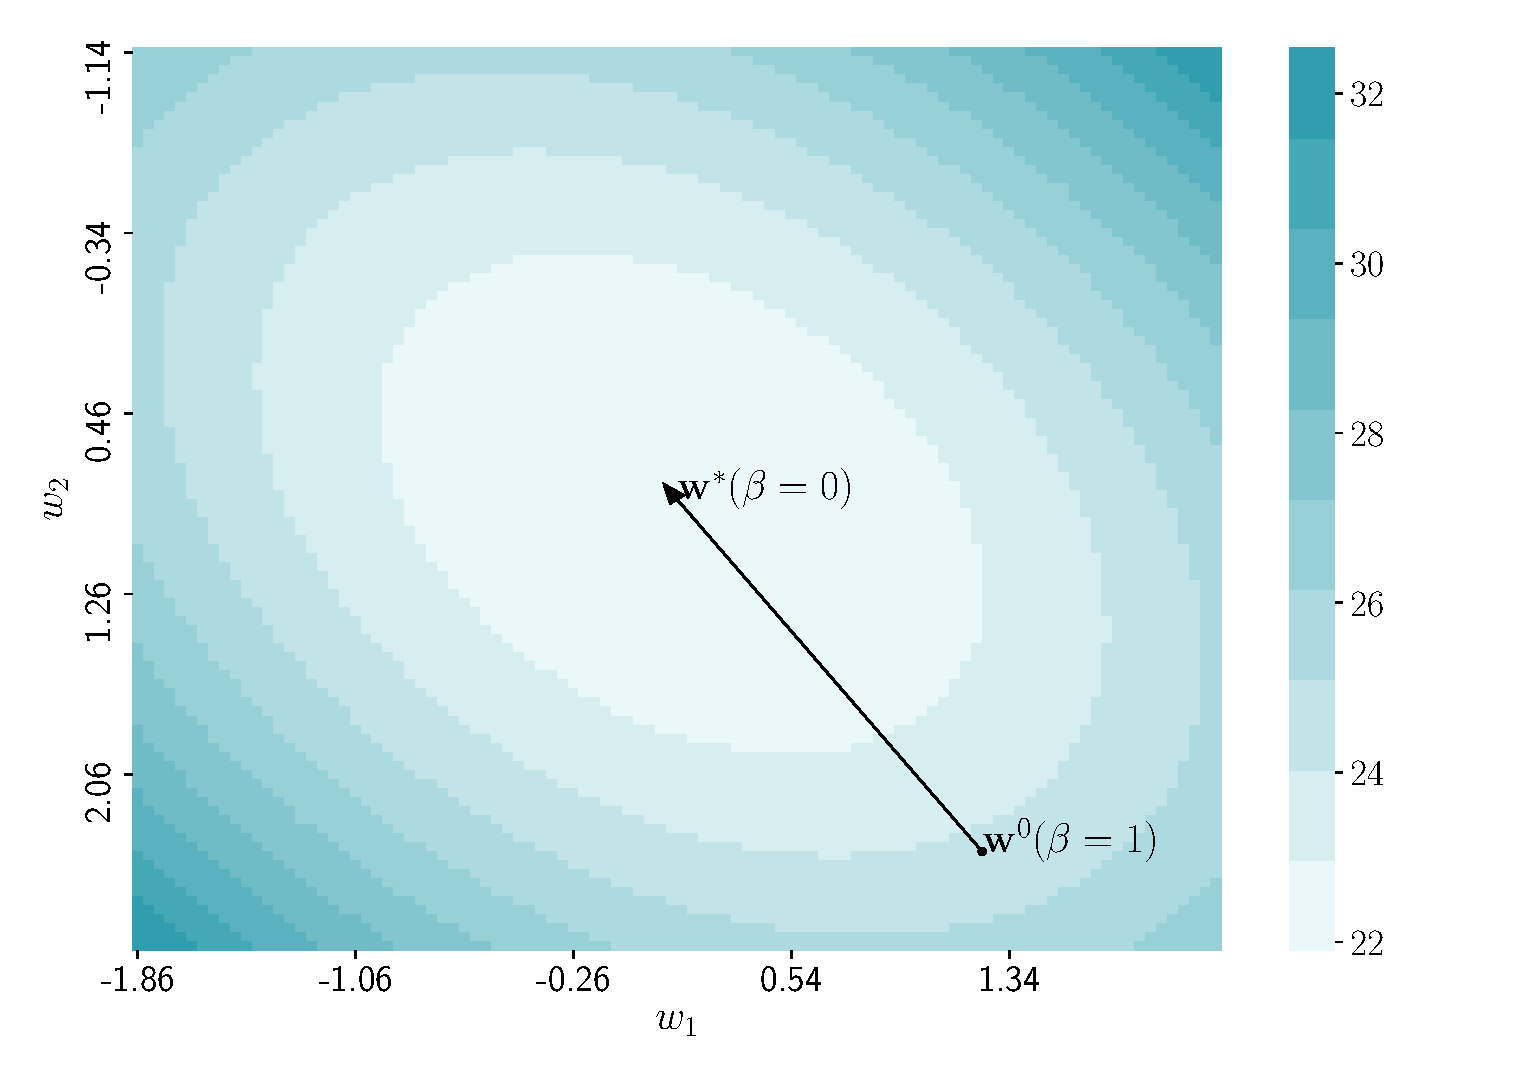
\includegraphics[width=0.8\linewidth]{figs/linear_error.eps}	 
		\caption{Error function landscape near optimal weight point for linear model.}
		\label{fig:linear_error}
	\end{figure}

	\begin{figure}[!h]	
		\centering
		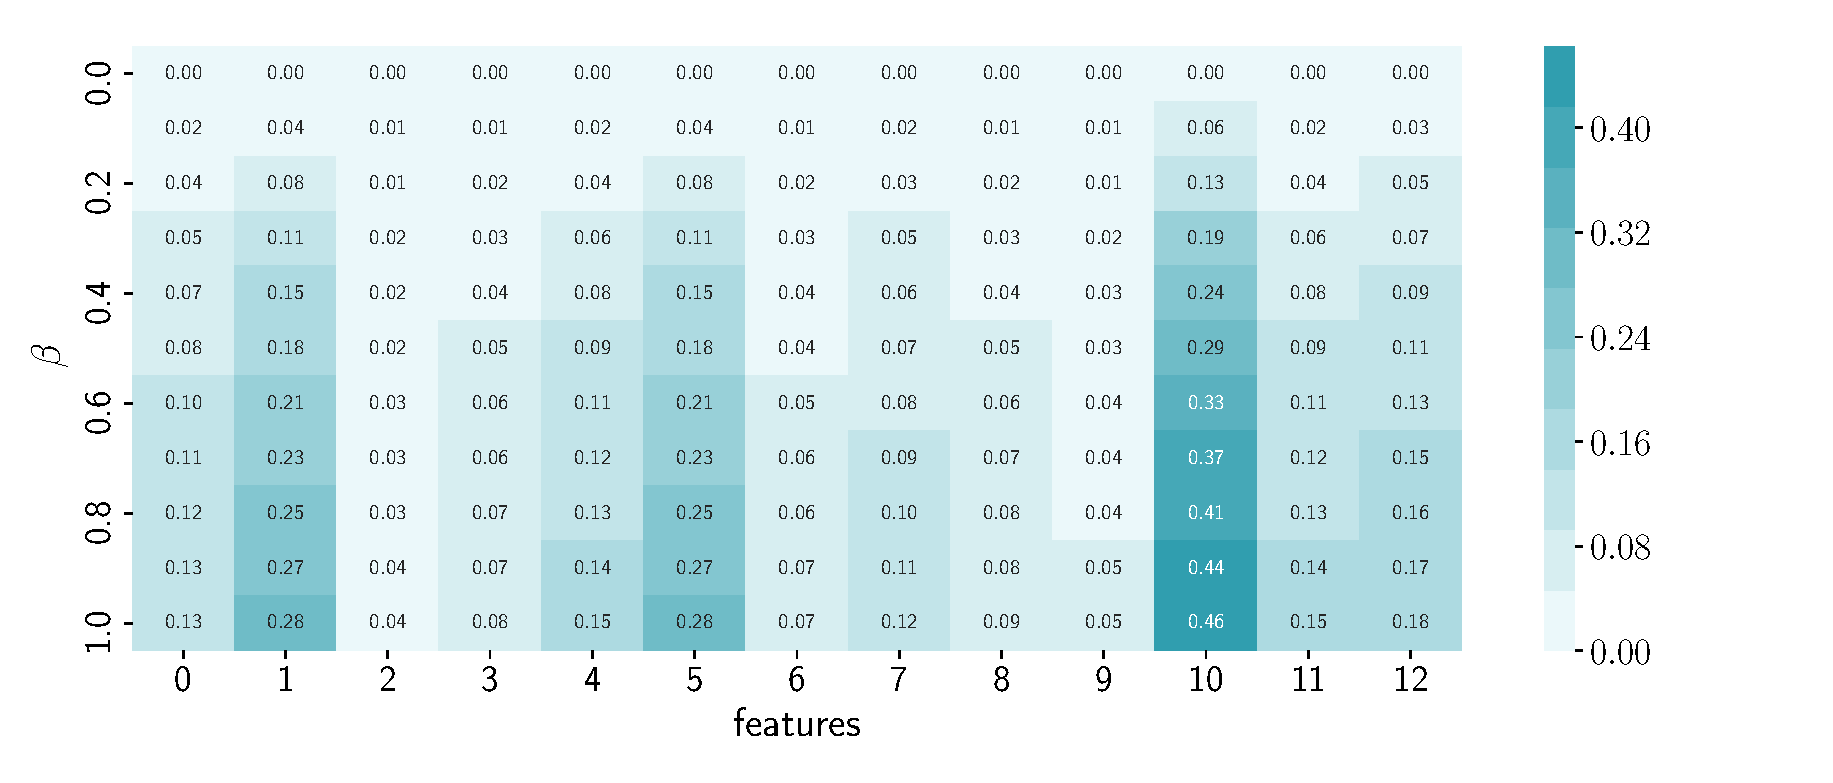
\includegraphics[width=\linewidth]{figs/linear_b_wrt_beta.eps}	 
		\caption{Relevance scores for linear model with respect to $\beta$ coefficient.}
		\label{fig:linear_b_wrt_beta}
	\end{figure}

	The landscape for the neural network model is more complex. We use only 2 hidden units to get not excessively complex model. The optimal weight vector $\bw^*$ is obtained by backpropagation optimization procedure. Figure~\ref{fig:neural_error} shows the error function on the grid of two neural network weights from~$\bW_1$. We use the same strategy to investigate how the linear term vector $\bb$ is changing moving from $\bw^0$ to $\bw^*$. The result are shown in the figure~\ref{fig:neural_b_wrt_beta}.
	

	\begin{figure}[!h]	
		\centering
		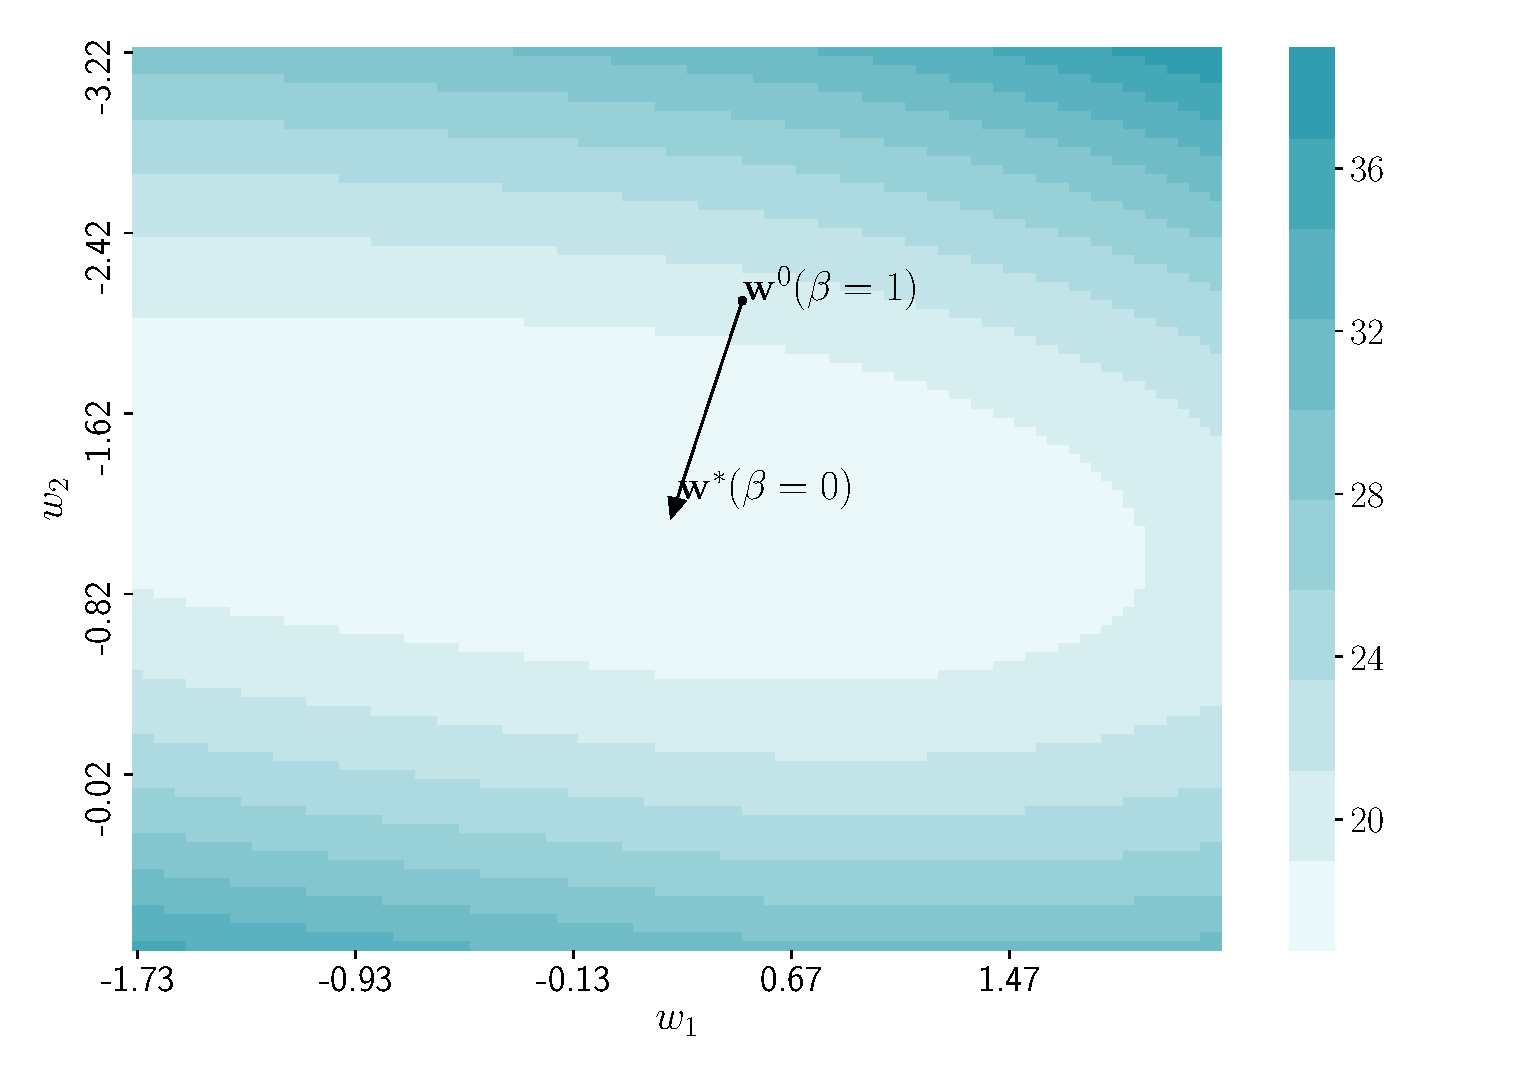
\includegraphics[width=0.8\linewidth]{figs/neural_error.eps}	 
		\caption{Error function landscape near optimal weight point for neural network.}
		\label{fig:neural_error}
	\end{figure}
	
	\begin{figure}[!h]	
		\centering
		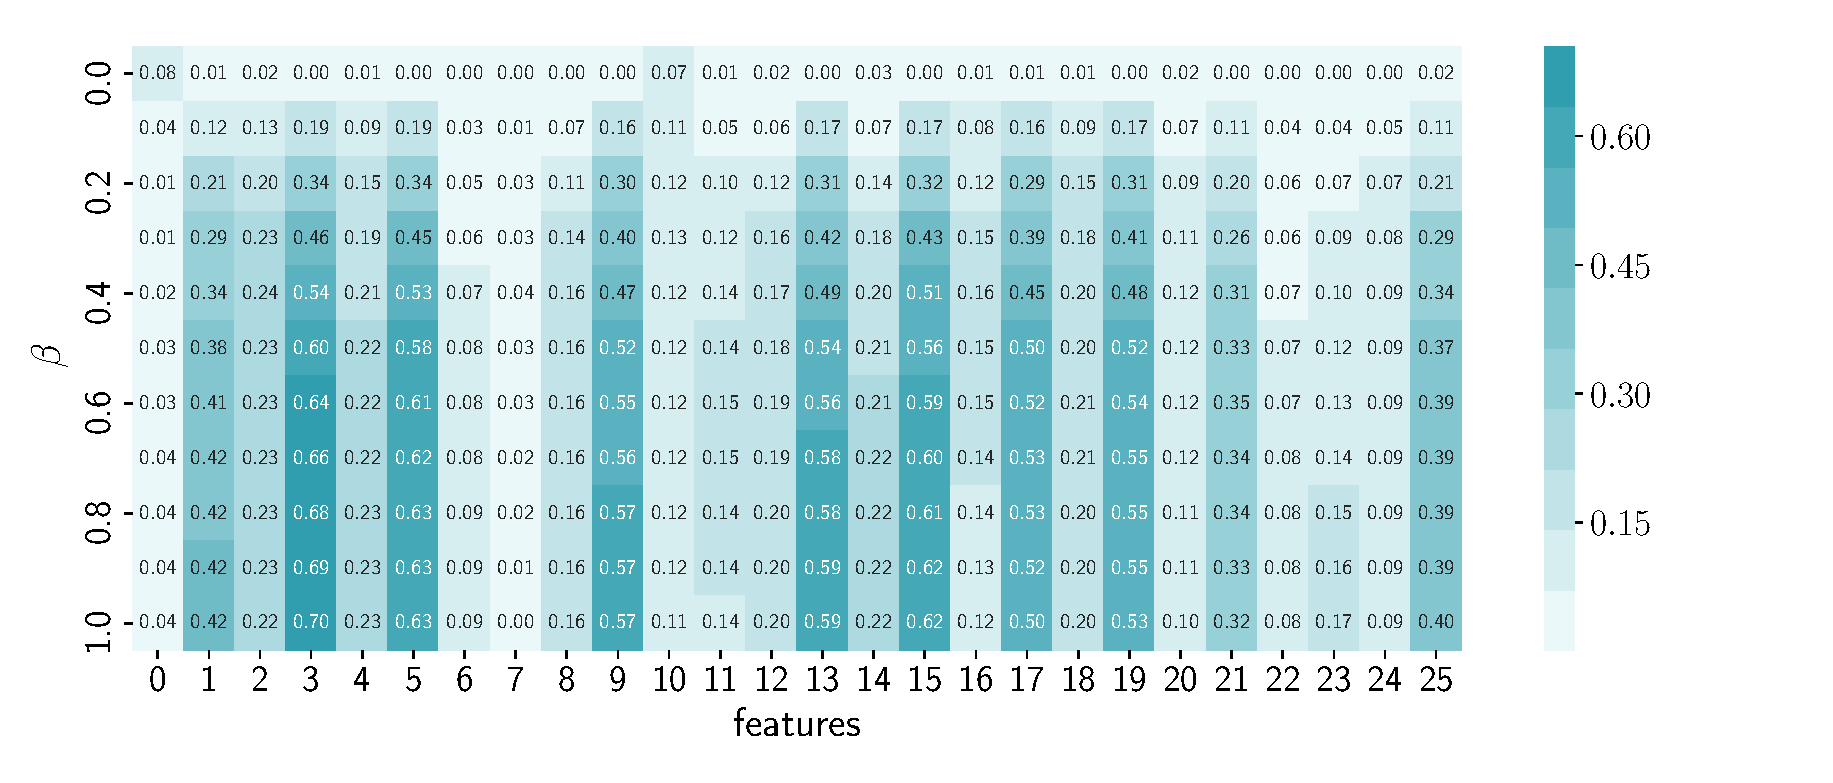
\includegraphics[width=\linewidth]{figs/neural_b_wrt_beta.eps}	 
		\caption{Relevance scores for neural network with respect to $\beta$ coefficient.}
		\label{fig:neural_b_wrt_beta}
	\end{figure}

	\begin{figure}[!h]	
		\centering
		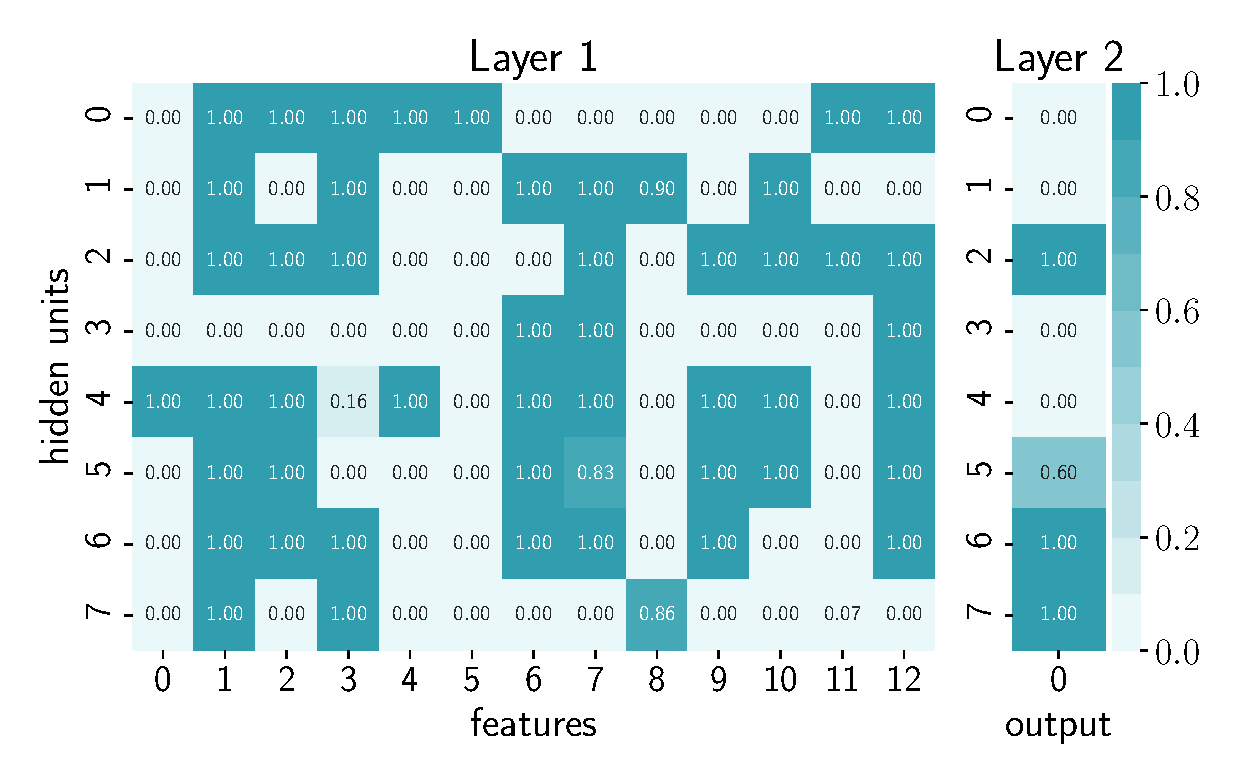
\includegraphics[width=0.8\linewidth]{figs/qpfs_nn_weight_maps.eps}	 
		\caption{Neural network weight scores maps for mutual information similarity coefficient}
		\label{fig:qpfs_nn_weight_maps}
	\end{figure}
				
   \newpage
   \hrulefill
  
	\end{document}